\chapter{METHODOLOGIES}

\graphicspath{ {./methodologies/} }
%%%%%%%% This line gets rid of page number on first page of text
\thispagestyle{empty}

%%%%%%%%%%%%%

\section{Method Selection}

The methodologies section covers methods chosen to investigate the research problem. I begin this section by restating the research problem and underlying assumptions underpinning this study: interpreting and understanding deep neural networks using interactive visualization, to inspire human curiosity and learning among the non-technical audience, as well as broaden people's access to interactive tools for deep learning.

\subsection{Scientific Methods}

The primary method selected for the research process is the scientific method. I selected this method as it involves careful observation and empirical study. Science involves empirical study of nature and scientific method has been the hallmark of several leading research in this inter-disciplinary field. Indeed, much like a child’s brain evolves to become a model builder and learn to learn, researchers in these field, over time, examined and pondered how to learn from nature by employing scientific method in their research process. 


Deep learning is essentially a method for machines to learn from data and classifying patterns that are loosely modeled on the way a biological brain learns to solve problems. This empirical method coupled with the detailed mathematical representation of the model and their numeric computation makes scientific method an ideal choice of method for this research. In this research, I use tools of scientific method for both performing experiments and raising application-agnostic questions of the inner working of the fundamental building blocks of the deep learning models, which ought to be examined with the tools of the scientific method to make sure we not only comprehend the effect, but also begin to understand the cause which is the raison d'\^{e}tre of science \cite{edsarx.1904.1092220190101}.

Although scientific method \cite{2016397} is widely discussed and written about, it remains simple in its core concept: observe a phenomenon of interest, formulate a mathematical model, verify how the model accounts for past observations, and use it to predict variants of the phenomenon and future observations. And, following Popper, models shall be readily abandoned if falsified by observed data. However, falsifiability is often largely insufficient: models based on distinct and perhaps incompatible assumptions may often be concomitantly supported by a specific dataset. It is thus necessary to identify extensions to existing measurements and examine where conflicting models may deviate appreciably from each other, and thereby provide grounds for additional testing and falsification.

The scientific method consists of two stages: (i) formulating hypotheses, and the (ii) testing them \cite{2016397}. What differentiates this from other forms of methods is the second stage: subjecting hypotheses to empirical testing by ascertaining whether or not predictions derived from hypotheses are borne out in relevant observations and experiments. Hypotheses and assumptions are the initial stages of scientific inquiry because they incentivize seeking truth and a hint as to where to find it \cite{AYALA2016xi}.

The underlying principles of the scientific method \cite{gauch_jr_2012} are essential for evaluating the hypothesis, enhancing perspective, increasing productivity, and inspiring innovation. These principles include logic, probability, parsimony and hypothesis testing, as well as science's presuppositions, limitations, principles and bold claims of rationality and truth. Beyond such methodology, some practical issues are shared broadly across the sciences, such as implementing effective science education and relating the scientific enterprise to the humanities.

Additionally, I also employed other research methods to support our research processes, such as action as research, agile development and system design. The selection of a research methodology was dependent on the research question itself and how best it can be addressed: interpreting deep neural networks.

\section{Research Hypothesis}

While deep neural nets learn efficient representations and deliver superior performance, most users consider them as a ‘black-box’ system, due to their opaque nature and complex working mechanism. As in most cases, they learn representation and patterns that is difficult to extract and present it in a human-readable form. While this is true for certain types of deep learning models, it is not entirely true for an image recognition model because they are representation of visual constructs and abstracts which can be deconstructed to see what shapes and patterns were detected by the model at successive layers \cite{Zeiler} and how does that correlate to the prediction class at the output.

Typically a neural network is provided with an instance, for example, an image or audio segment, and it computes transformation on this instance at successive layers until it finally produces a probability value for a prediction. Inside the network, each neuron at each layer detects a specific feature through training and multiple epochs. The information flowing through the neural network is a set of numerical weights parameters, and connections that provides no direct clues as to how the task is performed or what is the correlation between inputs and outputs. Further the parameter selection is random and adjusted iteratively throughout the training process.

My analysis of previous work suggest that deeper representation in a CNN capture high level abstracts or visual concepts \cite{Zeiler}. More importantly convolutional layers naturally retain the spatial information of the input data which is otherwise lost in the fully connected layers. Thus I expect the last convolutional layer to retain better features, which is balanced between spatial information and class semantics. The neurons in the last convolutional layer mostly observe the class specific information in the image, such as object parts. Therefore, I use gradient descent to compute the gradient of the activation output of the last convolutional layer in CNN to understand the importance of each neuron for a class of interest. We use relevance heatmap visualization to highlight the importance of each neuron (channel or filter) and its correlation to the prediction made by the model.

Building upon this assumption, we formally setup our hypothesis as follows: Apply image localization and object detection technique to distinguish what part of an input image attributed most to the classification decision by the model. In other words, localization is a useful method to study which pixels in a given input has high activations or to what input neurons are most receptive to and how does that correlate to the class prediction.

Finally, with the growing complexity of the deep learning model, the critical need for understanding its inner working has increased. I postulate interactive visualization is a potentially a powerful techniques to fill such a critical need. It can be used to deconstruct the problem of black-box system and able to inspect what features the network has learned, patterns discovered by filters and uncover other hidden structures in the data.

%visualization is a potentially a powerful techniques to fill such a critical need that can be used to see through the black box model and deconstruct it to understand what features the network has learned during inference.

% In deep learning visualization research, a large body of work is dedicated to visualizing particular neurons or neuron layers [1], [19]–[20][21][22][23][24] and learned parameters, our work chose to focus on collective output corresponding to the predicted class

\section{Design Goals}

Besides model complexity, the problem of trust and transparency has been receiving more attention lately for deep neural networks and other non-linear models \cite{edseee.839741120170101} \cite{edseee.863755220180101} \cite{S003132031630358220170501}. As a result, several methods have been developed to interpret what a deep neural network (DNN) has learned. A large section of work in DNN interpretability is dedicated to visualizing specific neurons or the layers. This work focuses on a method that can visualize the impact of particular regions of a given input instance on the prediction or the desired class of interest.

\begin{figure}[htbp]
\centering
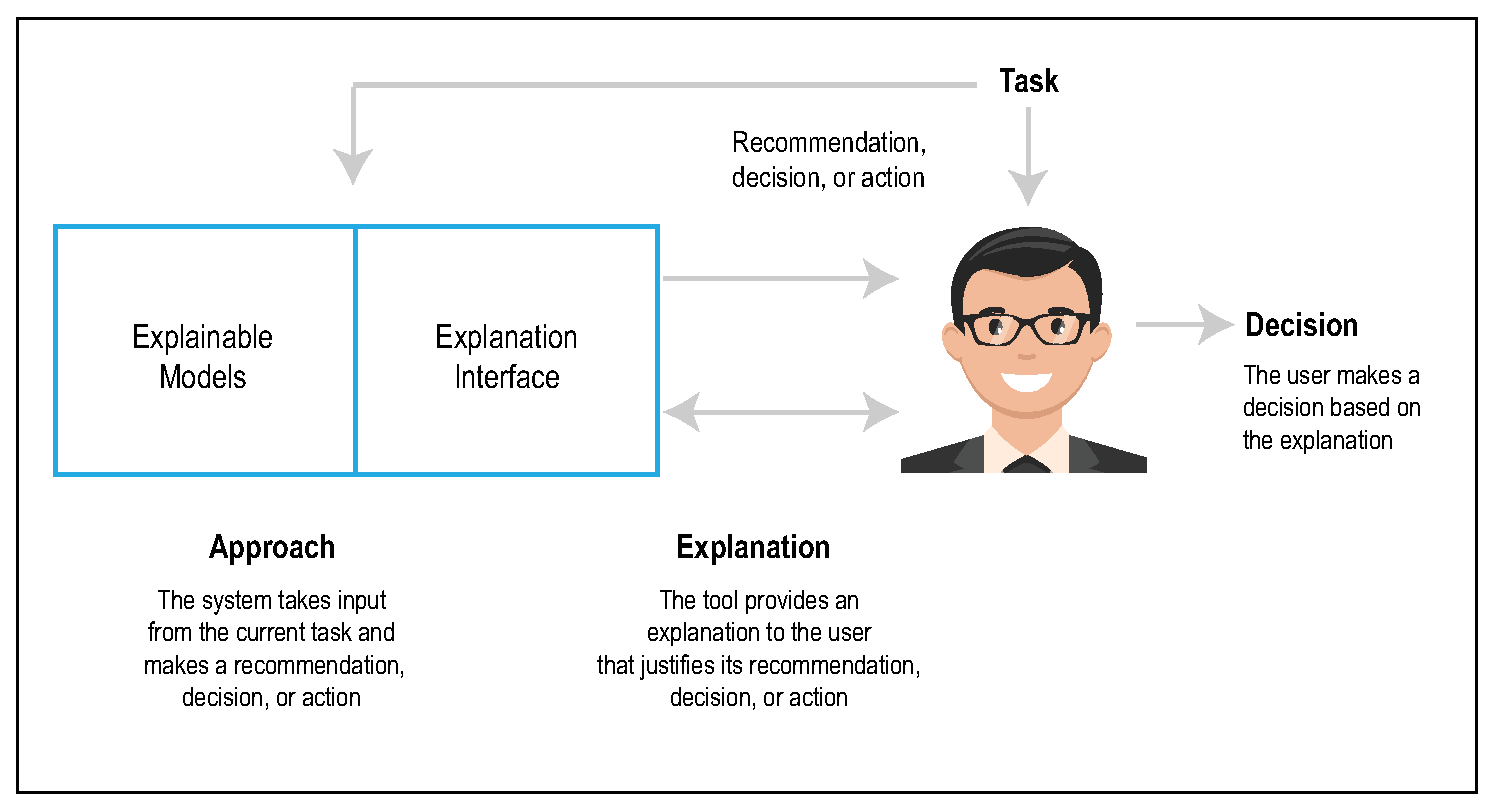
\includegraphics[width=0.85\textwidth]{images/xai-1.eps}
\caption{Explanation Approach}
\label{fig:explanation-approach}
\end{figure}

The goal is to build an interactive visualization tool to interpret a visual classifier model and provides explanation to the end user using visual evidence that justifies its recommendation, decision or action. I use the explanation approach in Figure 3.1 as the guiding principle to design and develop the explanation interface of the prototype.  The prototype objective can be summarized mainly as (i) Provide visual explanation that justifies model prediction or decision to non-specialist (ii) Education and communication for non-technical audience and (iii) broaden people's access to interactive tools for deep learning.

The prototype is intended and designed for people with a non-technical background to interact with and visually understand the decision of an image classifier. The top-level intent is to develop a set of utilities or toolkit as the first step towards building a robust explanation framework that can make any visual classifier more interpretable and explainable for the end user.


\section{DeepViz - Visual Exploration Tool}

\begin{figure}[htbp]
\centering
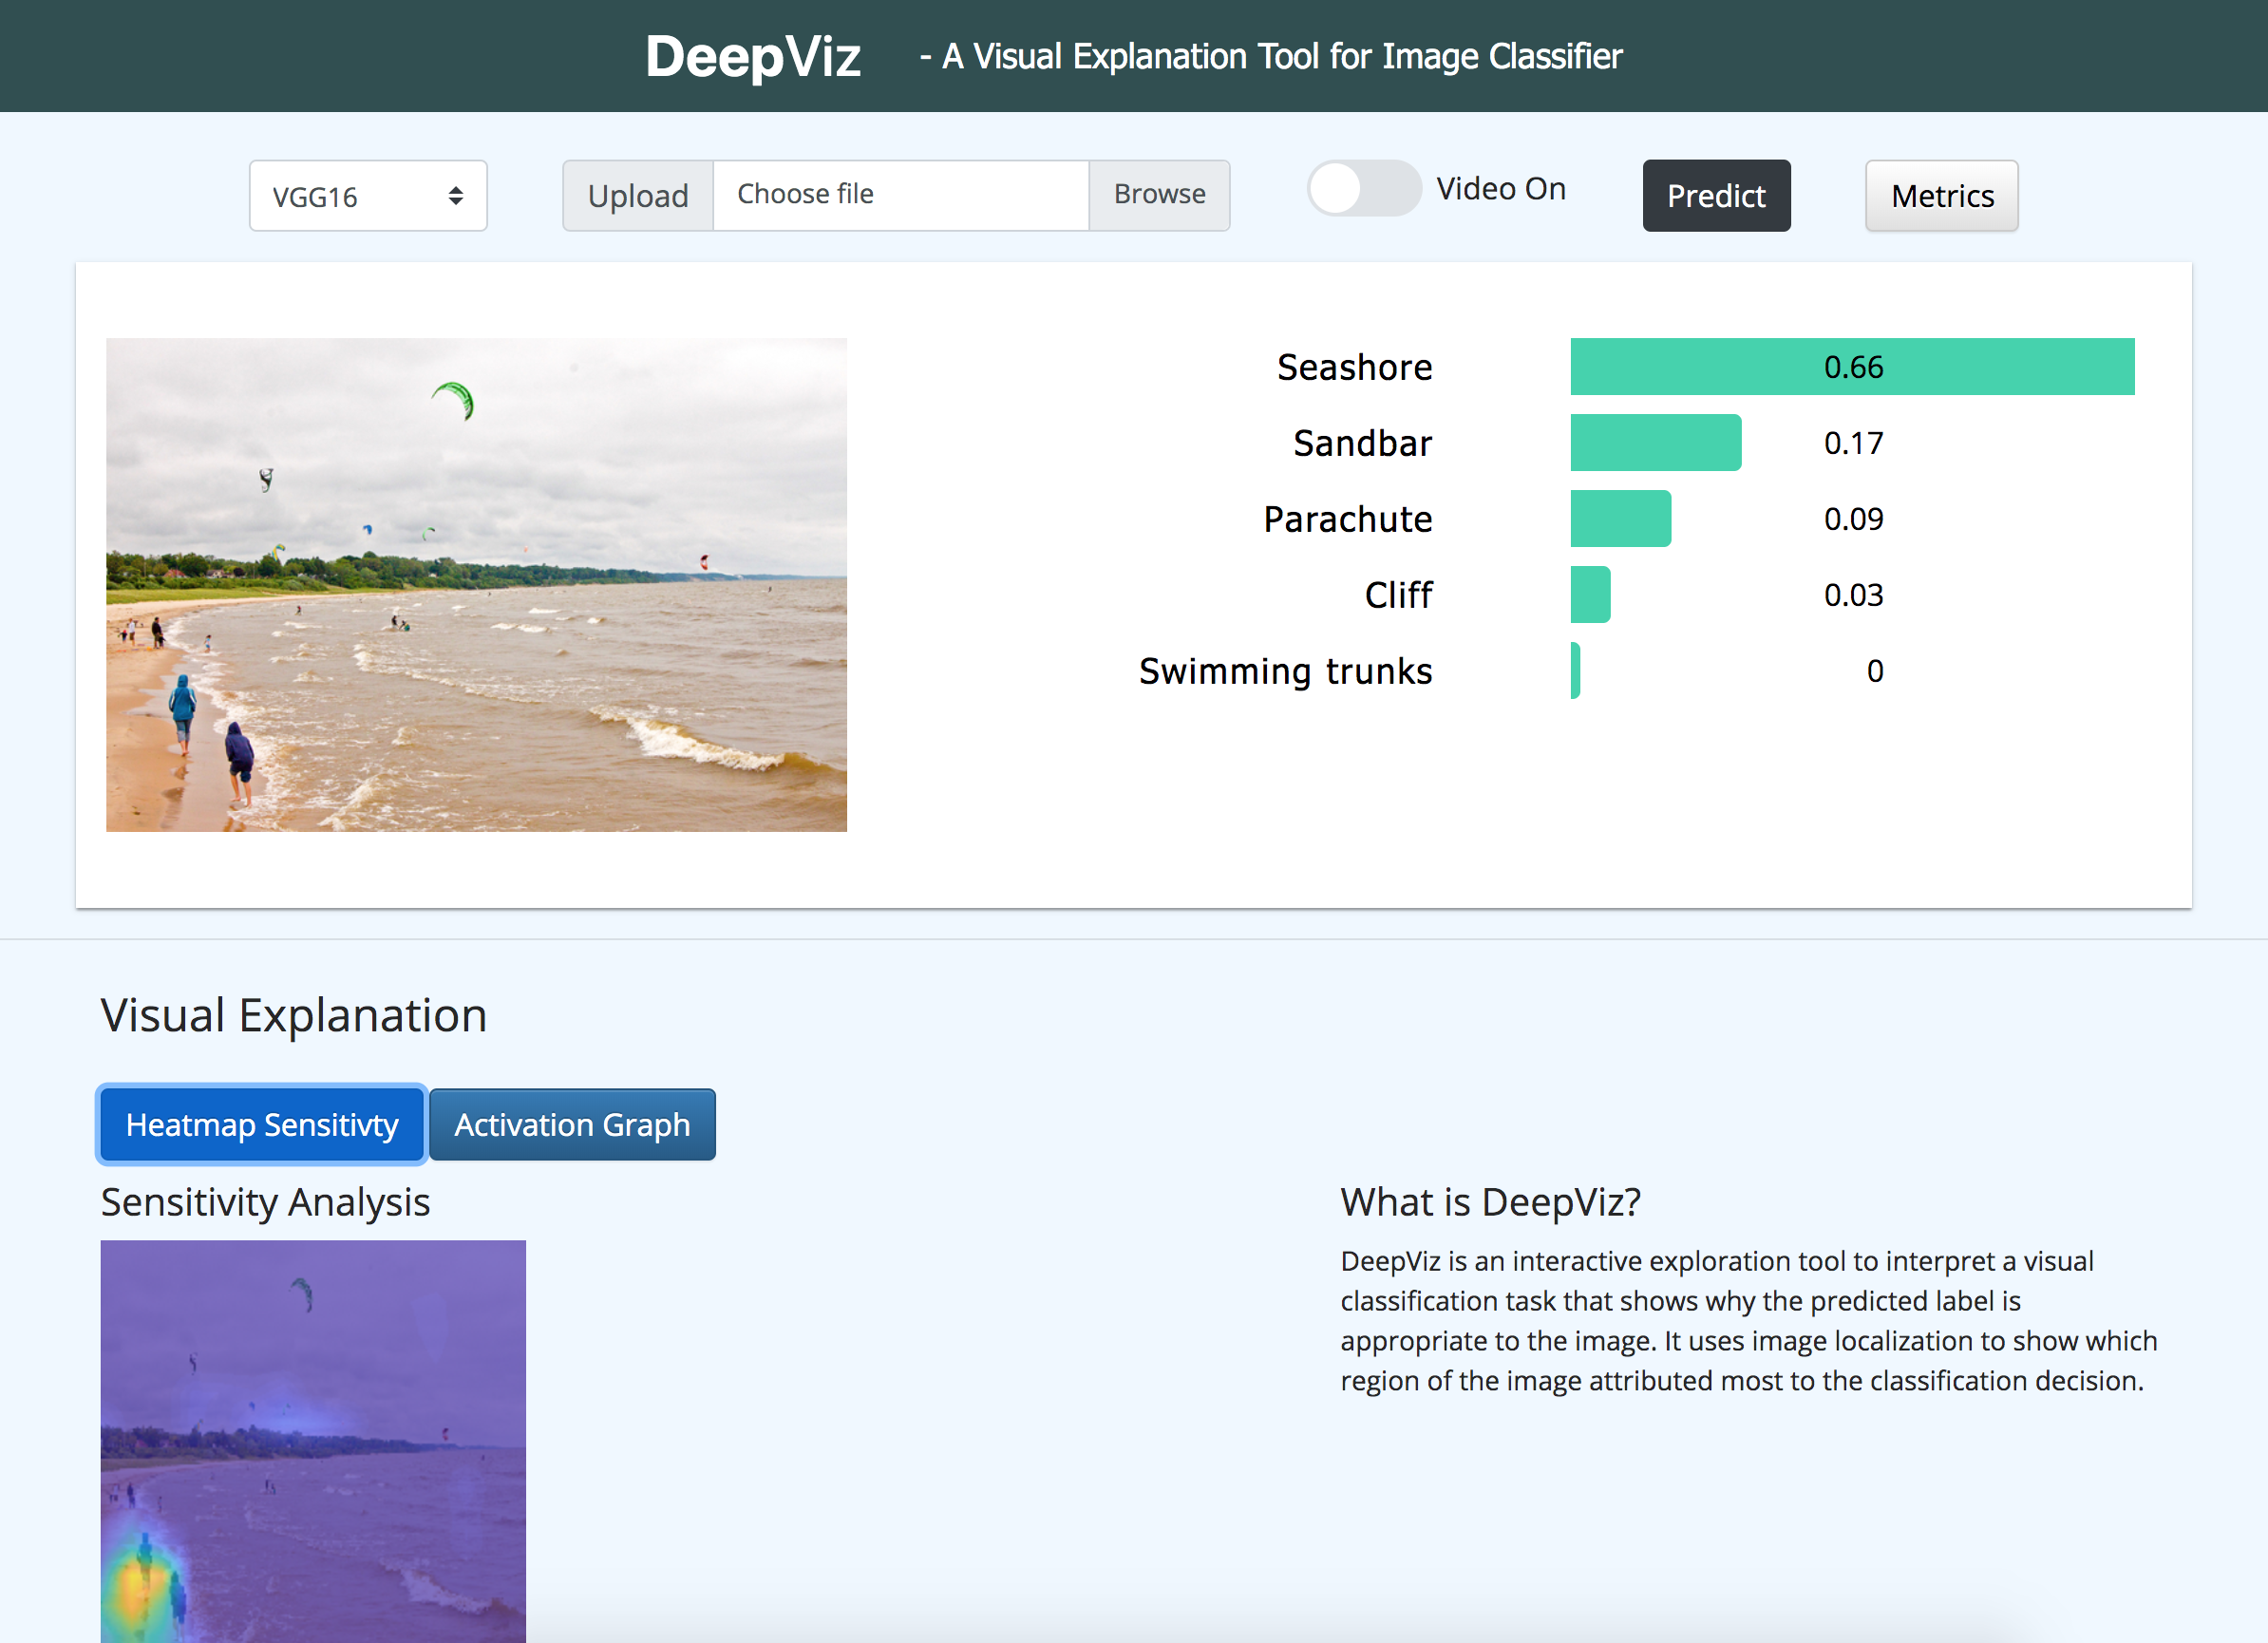
\includegraphics[width=0.90\textwidth]{images/DeepViz001.png}
\caption{Visual Explanation Tool}
\label{fig:DeepViz - Visual Explanation Tool}
\end{figure}

DeepViz serves as a visual exploration tool to enables interactive and explorable explanations of the model. It utilizes visualization technique that focuses on the class differential properties of the visual object and help end user understand the the model inference. The tool also visualizes the intermediate output of the network as a directed graph displaying a hierarchical representation of input transformation.

Firstly, When an image is submitted, DeepViz predicts a class label and then shows why the predicted label is appropriate for the image using relevance heatmap. This method is useful to highlight which part of the image is most relevant to the classification decision. The second method is an feature activation graph that displays what features a neural network has learned and how the network builds their internal representation of  features detected by the network during the inference process. Secondly, DeepViz produces an activation graph visualizing the the feature maps that are output by intermediate layers in the network. This graph visualization outlines how an input is decomposed into the various filters learned by the network.

\section{Design Approach}

\begin{figure}[htbp]
\centering\textbf{}
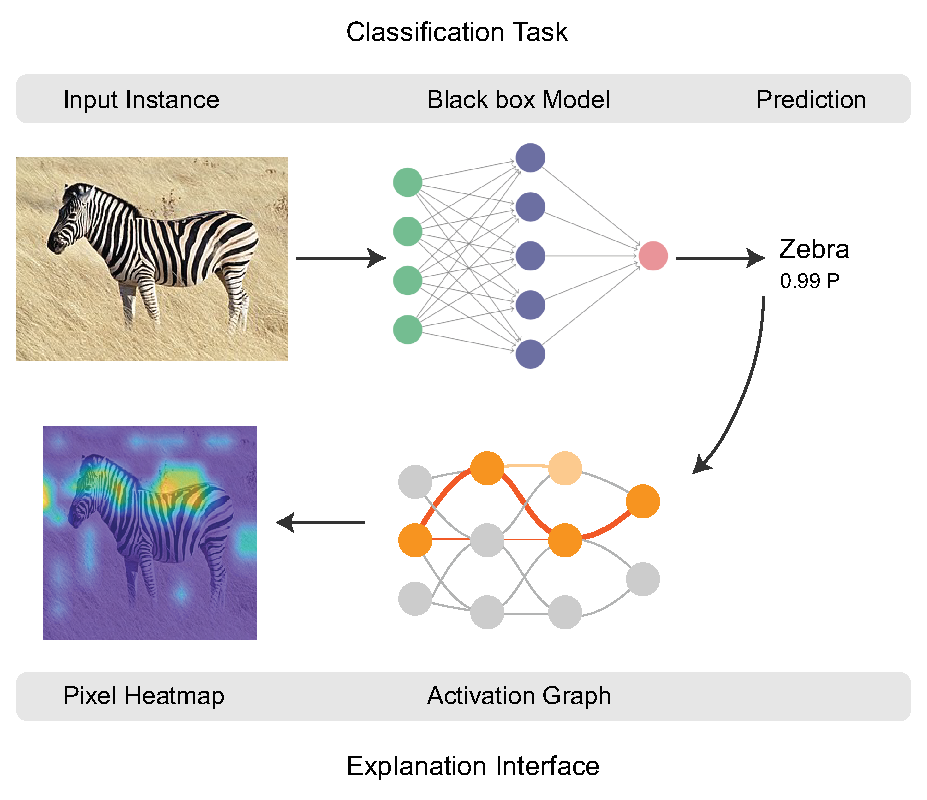
\includegraphics[width=0.80\textwidth]{images/method-schema-copy.eps}
\caption{Design Approach}
\label{fig:design-approach}
\end{figure}

This section introduces two visualization techniques implemented in the prototype for interpreting and exemplifying the prediction of an image classifier model.

\subsection{Sensitivity Analysis}

Sensitivity Analysis visualizes a heatmap of the activation output corresponding to the predicted label. This method is useful for interpreting which part of an input image led the model to its final classification decision. It localizes the class discriminative region in the image by generating a heatmap superimposed on the input image. It highlights the discriminating region corresponding to the desired class clearly.

For instance, when an image is submitted, the model predicts the class. The input image is correctly classified as "bee-eater". In order to understand why the model arrived at this decision, the tool generates a heatmap that visualizes the importance of each pixel in the input image for the prediction of that class. In this example, the bee-eater's beak and the neck are the basis for the model's decision. With the heatmap,user can verify that the model works as intended.

The tool uses localization to know what region in the image attributed most to the classification decision. This helps identify individual pixels in the input image that had the highest activations. Localization, in the context of CNN, is a task to localize objects in images using only whole image class labels. It indicates where the model has to look to make a specific decision. It identifies pixels which are pivotal for the prediction object.

I use Class Activation Mapping approach (CAM) to obtain the localization map. I focused on the output of the last convolutional layer because it detects the high level features and differential to the predicted class. Therefore, I computed the value of the activation output of the last convolutional layer, and then computed the gradient of the probability score of the class with respect to the logits or activation output of the last convolutional layer. This step helps capture the importance of the feature map for a targeted class. The gradient value is pooled within each filter by taking the global average mean. The resulting value is then multiplied with the activation output of the last convolutional layer for the weighted combination. The resulting value is averaged and all the filters are collapsed to create a heatmap vector. This is followed by ReLU (Rectified Linear Unit) activation in order to discard the negative values from the heatmap and normalize them. The heatmap vector is resized to match the size of the input image. An RGB colormap is applied to the heatmap vector to transform the 1-channel greyscale image into a color image. Then the color heatmap is overlaid on top of the input image to form the final output.

\subsection{Feature Activation Graph}

A feature activation graph visualizes the intermediate activations of the network. It takes the values of the activation output of all the convolutional layers and produces a directed acyclic graph. The output of the layer is actually the sum of the output of the activation function of all the channels in that layer. The graph decomposes the activation output at every layer into a distribution of channels per layer.

Visualizing intermediate activations helps display the feature maps produced as output by various convolution and pooling layers in a network, given a certain input. This gives an overview into how an input instance is decomposed into the different filters learned by the network. These filters consist of 3 dimensions (width, height and depth), where each channel encodes relatively independent feature. Thus we visualize these feature maps for every channel as a 2D image in individual vertices.

The direction of the graph is from bottom to top corresponding to lower level to higher level. Each level represents a convolutional layer, where each vertices represents an individual channel. An edge connecting two vertices represents the weight between neurons in successive layers. User can explore the edges to discover what the network detects at each layer as it propagates the activation output forward. This step helps user understand when fed with an input image, how successive layers of the network transformed the input image. This also gives an idea of the meaning of the individual network filters.

Although VGG16 model has 18 such hidden layers with channels ranging from 64 to 512, we have limited the number of layers and channels in our view to only 8 in order to maintain optimum performance of the application given the rendering effort is expensive to render all channels.

\section{Technical Design}
The following segment provides an overview of the technical design and resources required for the successful development of the prototype. It provides a high-level overview of the components in scope, functionality, dataset and environmental setup.

\subsection{Client-side Neural Network}
Developing AI applications using modern deep learning framework is a non-trivial task. Normally these frameworks and libraries are leveraged by native applications that run on a native platform environment such as Linux, Windows, MacOS/iOS and Android. Thus most production-level libraries are developed for and written in Python, Java and C++.

Developing machine learning application that is cross-platform and portable on multiple devices is not easy. The development of a native application is an intricate and time-consuming process. It is particularly complicated for mobile applications as the app vendors usually need to develop and maintain both iOS and Android version, in addition to the desktop application.

Compared to the native application, client-side applications can make the portability issue simpler for the cross-platform. The sample implementation of deep learning powered web application can be deployed on multiple platforms regardless of operating systems, hardware or device types.

Deep learning in the browser is at the experimental stage and recently several JavaScript-based deep learning frameworks have been introduced, making it possible to perform several deep learning tasks directly on the browser. Some of the supported features include model training, importing pre-trained models, transfer learning and inferences.

However, there is a debate on the feasibility and effectiveness of the web-based deep learning applications. One one hand, those who object think browsers are not primed for running deep learning tasks and its merely impractical due to the poor performance of client-side scripting and limitations imposed by the browsers. On the other hand, advocates think that the browser is an ideal platform for realizing client-side machine learning that allows highly rich interaction and improves personalization for end users. The benefits include but not limited to faster user interaction, preserving data privacy, lower back-end payload, reduced data transfer and performance latency of HTTP client-server communication.

\subsection{Supported Browser Features}
I analyzed the modern browser support for machine learning tasks and taken into consideration the factors that may affect the efficiency when building and deploying deep learning application on the web. One of them is the debugging capability to support model and data inspection when running deep learning tasks.

Further, in-browser deep learning allows users to use local data and then train the model directly in the browser, meaning there is no back-end end or server is necessary. 
\subsection{Model Selection}

As the model selection is the centerpiece of the data science workflow, I evaluated a set of candidate pre-trained models for my classification project by running a series of study and experiments. Specifically, I created a special Python script that can load any of these pre-trained network architectures from disk using Keras, and then classify a set of sample images. I ran the experiments on models namely, MobileNet, Inception V1, Inception V3, VGG16 and VGG19 and compared them in terms of performance, accuracy, network architecture and size of the learned parameters. VGG16 and VGG19 have better accuracy than other models and both are trained on ImageNet database. The “16” and “19” stand for the number of hidden layers in the network. Due to their depth and number of fully connected units, VGG16 is 533MB and VGG19 is 574MB in size. This experiment also helped assess if the data collected for inference is suitable for the classification task. I took into account the hyperparameter setting and other configuration details required to evaluate during the inference process if required. We tested the compatibility of the model with the available dataset. Based on my evaluation and initial experiments, I selected VGG-16 as the primary model for the prototyping phase.

\begin{figure}[htbp]
\centering
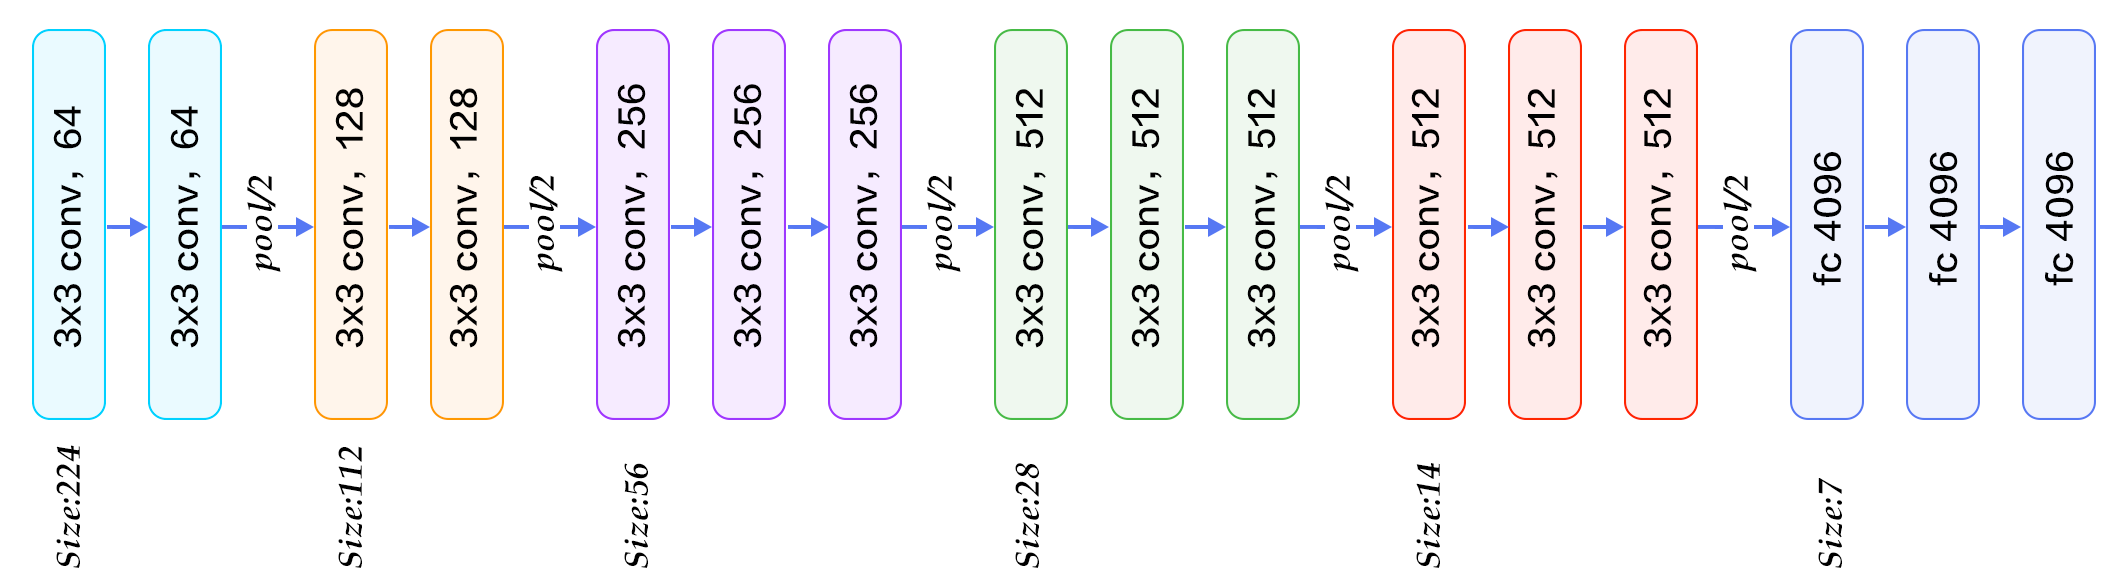
\includegraphics[width=1\textwidth]{images/cnn-vgg16-1.png}
\caption{A schematic view of Visual Geometry Group 16 Model}
\label{fig:CNN-1}
\end{figure}

VGG-16 is based on convolutional neural network model proposed by the Visual Geometry Group from the University of Oxford in the paper “Very Deep Convolutional Networks for Large-Scale Image Recognition” \cite{2014arXiv1409.1556S}. The model achieves 92.7\% top-5 test accuracy in ImageNet, which is a dataset of over 14 million images belonging to 1000 classes. It was one of the famous model submitted to ILSVRC-2014 competition. Ths list of hidden layers can be seen in the table \ref{table:vgg16-layer}. This model is used as the backbone network in our project.

\subsection{Dataset}

ImageNet is a massive database of image collection that consist of over 15 million labeled high-resolution images belonging to roughly 22,000 categories \cite{edsarx.1409.057520140101}. These images were downloaded from Google image search and labeled by humans using Amazon's Mechanical Turk crowd-sourcing tool in 2012. It took about two and half years to label all the images. 

The labeled dataset was first introduced in a competition called the ImageNet Large-Scale Visual Recognition Challenge (ILSVRC). The competition used a subset of ImageNet with around 1000 images in each of 1000 categories. In total, there are 1.2 million training images, 50,000 validation images, and 150,000 testing images. To maintain consistency of resolution, images have been down-sampled to a fixed resolution of 256x256 dimensions.
    
\subsection{Framework Selection}

To develop client-side deep learning application, I surveyed the open source machine learning frameworks for the web: TensorFlow, Keras, and WebDNN. Based on my assessment and feedback from the developer community, I selected TensorFlow in Python and TensorFlow.js for the prototype development. I also use JavaScript ES6 and Node.js for server side processing and environmental setup.

I found TensorFlow.js as a better choice for training and inferring deep learning models on the browser. While several other open source JS platforms for machine learning have appeared in recent past, I noticed TensorFlow.js as feature-rich and well-documented when compared to other web libraries. Further, TensorFlow.js takes advantage of GPU processing power to accelerate deep learning tasks on browsers via WebGL \cite{Ma2019}, which is an important criteria for my tool that runs inference on a vision based model. WebGL is a back-end compute and a JavaScript API for rendering interactive 2D and 3D graphics within web browser without the use of additional plug-ins.

Since both client-side and server-side framework are part of the TensorFlow ecosystem, I can easily access APIs that are compatible with either ones. This also makes model conversion easier and allows for models to be ported between Python and JavaScript ecosystems \cite{Smilkov2019}.

\section{System Design}

As one of my goal for the prototype is to broaden people's access interactive tools for deep learning, and that the tool is targeted towards non-technical audience, DeepViz is a web-based interactive visualization tool that can be accessed from any modern web-browser. 

The development environment for the client side application is setup using JavaScript ecosystem and W3C web standards. DeepViz uses the web technologies: HTML, CSS, JavaScript ES6 and SVG. Node.js is used for back-end scripting for JavaScript ecosystem. For client-side visualization, I use SVG and D3.js for rendering vector graphics for the graph views. I also use the Lucid library for experimenting and testing feature visualizations in VGG16 model.

I leverage transpilers to transform code written in JavaScript ES6 into standard ES5 JavaScript that is executable in any browser. I also use bundling and tooling for local development and prototype deployment on the server.

\subsection{Environment Setup}

The development environment for the client side application is setup in Node.js environment. Its also used for tooling and bundling production deployment assets. For the back-end deep learning framework, we executed all our code on the workstation hosted on the virtual server provided by the NYU High Performance Computing services. 

%For the back-end deep learning framework, we executed all our code on an NVIDIA DGX, a workstation with 4 GPUs, with 16GB of RAM, 10 CPUs and 540GB of RAM.